\section{Wärmetransport}
\subsection{Wärmestrahlung}
\begin{flushright}
	$\boxed{\textbf{Buch S. 331}}$
\end{flushright}

 siehe \cbl{\hyperref[subsec:Strahlung]{Anhang - Strahlung}}

\subsection{Wärmeleitung - Fläche}
\begin{flushright}
	$\boxed{\textbf{Buch S. 325}}$
\end{flushright}

$$\boxed{Q = \frac{\lambda A \Delta T}{l}}$$

\subsection{Wärmedurchgang}
\begin{flushright}
	$\boxed{\textbf{Buch S. 328 \& 329}}$
\end{flushright}

\begin{center}
	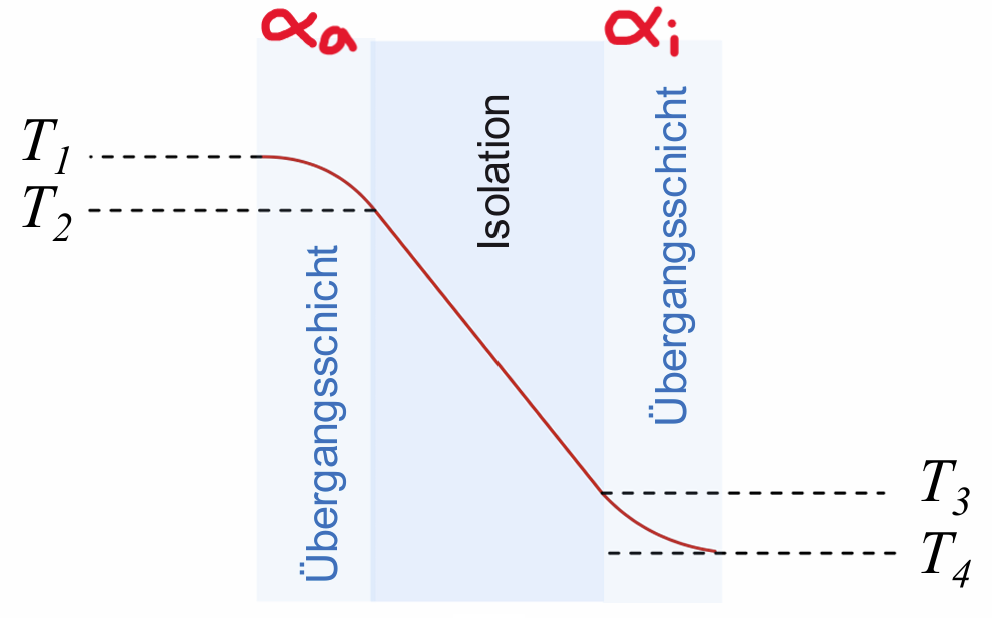
\includegraphics[width=0.5\columnwidth]{images/Waermetransport.png}
\end{center}

Der Wärmeübergangskoeffizient beschreibt den Wärmeübergang an einer Grenzfläche und hängt von den involvierten Materialien / Gasen ab. 

$$\boxed{j_a = \alpha_a \cdot \left( \underbrace{T_1}_{Fl.~~aussen} - \underbrace{T_2}_{Wand}\right)} \qquad \boxed{j_i = \alpha_i \cdot \left( \underbrace{T_3}_{Wand} - \underbrace{T_4}_{Fl.~~innen}\right)}$$

Für das ganze System ergibt sich die Wärmestromdichte (mit Wärmedurchgangszahl $k$)

$$ \boxed{ j = k_Q \cdot (T_1 - T_4) = k \cdot \Delta T} \qquad \qquad
\boxed{k = \frac{1}{\frac{1}{\alpha_i} + \frac{d}{\lambda} + \frac{1}{\alpha_a}}} $$

$$\boxed{k = \frac{\lambda}{d} \left( 1 + \frac{\lambda}{d \alpha_{\text{in}}} + \frac{\lambda}{d \alpha_{\text{out}}} \right)^{-1}}$$
\renewcommand{\arraystretch}{1.3}
\begin{tabular}{c l c}
	$j$ 						& Wärmestromdiche 			& $[j] = \frac{\watt}{\meter^2}$ 								\\
	$\lambda$ 					& Wärmeleitfähigkeit 		& $[\lambda] = \frac{\watt}{\meter \, \kelvin}$ 				\\
	$\alpha_i$ 					& Wärmeübergangszahl innen 	& $[\alpha_i] = \frac{\watt}{\meter^2 \, \kelvin}$				\\
	$\alpha_a$ 					& Wärmeübergangszahl aussen & $[\alpha_a] = \frac{\watt}{\meter^2 \, \kelvin}$				\\
	$T_1$ 						& Aussentemperatur 			& $[T_1] = \kelvin$ 											\\
	$T_2$ 					& Temperatur Wand aussen 	& $[T_2] = \kelvin$ 											\\
	$T_3$ 					& Temperatur Wand innen 	& $[T_3] = \kelvin$ 											\\
	$T_4$ 						& Innentemperatur 			& $[T_4] = \kelvin$ 											\\
	$k_Q$ 						& Wärmedurchgangszahl gesamt		& $[k] = \frac{\watt}{\meter^2 \, \kelvin}$						\\
	$d$ 						& Dicke der Wand 			& $[d] = \meter$
\end{tabular}
\renewcommand{\arraystretch}{1}

\vspace{0.2cm}

\textbf{Hinweis:} Je besser das Material isoliert (kleiner $k$-Wert) oder je geringer der Temperaturunterschied zwischen innen und aussen ist, desto weniger Wärmeenergie zwängt sich pro Quadratmeter durch die Wand.

\subsubsection{Wärmedurchgang komplett}

Der komplette Wärmedurchgang leitet sich her durch die \textbf{Erhaltung der Wärmestrondichte $\bm{j}$} und errechnet sich mit:

$$ \boxed{\text{n Schichten:} \quad \frac{1}{k_{\rm tot}} = \frac{1}{\alpha_i} + \sum_x  \frac{1}{k_x} + \frac{1}{\alpha_a} } $$

$$ \boxed{\text{zylindrisch:} \quad \frac{1}{k_{\rm tot}} = r_a \Biggl( \frac{1}{\alpha_i \cdot r_i} + \sum_x \frac{1}{\lambda_x} \cdot \ln \Biggl( \frac{r_{xa}}{r_{xi}} \Biggr) + \frac{1}{\alpha_a} \cdot \frac{1}{r_a} \Biggr) } $$


\renewcommand{\arraystretch}{1.3}
\begin{tabular}{c l c}
	$k_x$ 		& Wärmedurchgangszahl $x$-te Schicht 	& $[k_x] = \frac{\watt}{\meter^2 \, \kelvin}$ 		\\
	$\alpha_i$ 	& Wärmeübergangszahl innen 				& $[\alpha_i] = \frac{\watt}{\meter^2 \, \kelvin}$	\\
	$\alpha_a$ 	& Wärmeübergangszahl aussen 			& $[\alpha_a] = \frac{\watt}{\meter^2 \, \kelvin}$ 	\\
	$r_i$ 		& Innenradius Rohr 						& $[r_i] = \meter$									\\
	$r_a$ 		& Aussenradius Rohr 					& $[r_a] = \meter$									\\
	$\lambda_x$ & Wärmeleitfähigkeit 					& $[\lambda] = \frac{\watt}{\meter \, \kelvin}$
\end{tabular}
\renewcommand{\arraystretch}{1}


\subsection{Wärme-Bedarf (Heizleistung)}

Der Wärme-Bedarf (=Heizleistung) setzt sich zusammen aus \textbf{Wärmeverlust durch Wärmeleitung} und durch
\textbf{Wärmeverlust durch Luftaustausch}: 

$$ \underbrace{\text{Wärmeverlust}}_{\substack{\dot{Q}}}  = \underbrace{\text{Heizleistung}}_{\substack{P}} $$
$$ \boxed{ P = \dot{Q}_{\rm tot} = \dot{Q}_W + \dot{Q}_L }  $$

\begin{minipage}{0.4\columnwidth}
	$$ \boxed{ \dot{Q}_W = A \cdot j = A \cdot k \cdot \Delta T } $$
\end{minipage}
\hfill
\begin{minipage}{0.4\columnwidth}
	$$ \boxed{ \dot{Q}_L = c_L \cdot \rho_L \cdot \dot{V} \cdot \Delta T} $$
\end{minipage}

$$ \boxed{ \text{allgemein:} \quad \dot{Q}_{\rm tot} = \sum_{i=1}^n  \Big[ (A_i \cdot k_i + c_L \cdot \rho_L \cdot \dot{V} ) \cdot \Delta T \Big] } $$


\renewcommand{\arraystretch}{1.3}
\begin{tabular}{c l c}
	$\dot{Q}_{\rm tot}$	& Totaler Wärmeverlust														& $[\dot{Q}_{\rm tot}] = \frac{\joule}{\second} = \watt$	\\
	$\dot{Q}_W$ 		& Wärmeleitung 																& $[\dot{Q}_W] = \frac{\joule}{\second} = \watt$			\\
	$\dot{Q}_L$ 		& Luftaustausch 															& $[\dot{Q}_L] = \frac{\joule}{\second} = \watt$			\\
	$k_i$ 				& Wärmedurchgangszahl $i$-te Schicht 										& $[k_i] = \frac{\watt}{\meter^2 \, \kelvin}$ 				\\
	$\dot{V}$ 			& Volumenstrom 																& $[\dot{V}] = \frac{\meter^3}{\second}$ 					\\
	$\rho_L$ 			& Dichte der Luft: $\rho_L = 1.2 \, \frac{\kilogram}{\meter^3}$				& $[\rho_L] = \frac{\kilogram}{\meter^3}$ 					\\
	$c_L$ 				& Wärmekapazität Luft: $c_L = 1000 \, \frac{\joule}{\kilogram \, \kelvin}$ 	& $[c_L] = \frac{\joule}{\kilogram \, \kelvin}$ 			\\
	$A$ 				& Fläche der Wärmeleitung 													& $[A] = \meter^2$ 											\\
	$\Delta T$ 			& Temperaturdifferenz 														& $[\Delta T] = \kelvin$
\end{tabular}
\renewcommand{\arraystretch}{1}


\subsection{Wärmeverlust durch Abstrahlung}

Durch Strahlung kann auch Wärme übertragen werden.

$$ \boxed{ j_{12} = c_{12} \cdot (T_1^4 - T_2^4) = \sigma \cdot \varepsilon \cdot (T_1^4 - T_2^4) }   $$

\renewcommand{\arraystretch}{1.3}
\begin{tabular}{c l c}
	$j_{12}$ 		& Wärme-Transport durch Strahlungsaustausch 														& $[j_{12}] = \frac{\watt}{\meter^2}$ 				\\
	$c_{12}$ 		& Strahlungsaustauschzahl 																			& $[c_{12}] = \frac{\watt}{\meter^2 \, \kelvin^4}$ 	\\
	$\sigma$ 		& Stefan-Boltzmann-Konstante $\sigma = 5.671 \cdot 10^{-8} \, \frac{\watt}{\meter^2 \, \kelvin^4}$	& $[\sigma] = \frac{\watt}{\meter^2 \, \kelvin^4}$	\\
	$\varepsilon$ 	& Emissionsverhältnis 																				& $[\varepsilon] = 1$
\end{tabular}
\renewcommand{\arraystretch}{1}

\subsection{Transportvorgänge}

\begin{minipage}[c]{0.48\columnwidth}
	\subsubsection{Diffusion}
	
	Transport von \textbf{Masse} 
	$$ \boxed{ j_D = -D \cdot \frac{\mathrm{dn}}{\mathrm{dx}} \qquad \quad  D = \frac{1}{3} \cdot \overline{v} \cdot \overline{\lambda} }  $$
\end{minipage}
\hfill
\begin{minipage}[c]{0.48\columnwidth}
	\subsubsection{Viskosität}
	
	Transport von \textbf{Impuls} 
	$$ \boxed{ \tau = - \eta \cdot \frac{\mathrm{dv}}{\mathrm{dx}} \qquad \quad  \eta = \frac{1}{3} \cdot n \cdot \overline{v} \cdot \overline{\lambda} \cdot \rho }  $$
\end{minipage}

\medskip

\renewcommand{\arraystretch}{1.3}
\begin{tabular}{c l c}
	$j_Q$ 					& Wärmestrom 																& $[j_Q] = \frac{\watt}{\meter^2}$ 			\\
	$\lambda_Q$ 			& Wärmeleitfähigkeit 														& $[\lambda_Q] = \frac{\watt}{\kelvin}$ 	\\
	$j_D$ 					& Diffusionsstrom 															& $[j_D] = ?$ 								\\
	$D$ 					& Diffusionskonstante 														& $[D] = \frac{\meter^2}{\second}$ 			\\
	$\tau$ 					& Schubspannung 															& $[\tau] = \newton$ 						\\
	$\eta$ 					& Viskosität	 															& $[\eta] = \pascal \, \second$ 			\\
	$n$ 					& \crd{Molekül-Dichte} 														& $[n] = \frac{1}{\meter^3}$				\\	
	$\overline{v}$ 			& Mittlere Geschwindigkeit 													& $[\overline{v}] = \frac{\meter}{\second}$	\\
	$\overline{\lambda}$ 	& Mittlere freie Weglänge 													& $[\overline{\lambda}] = \meter$ 			\\
	$f$ 					& Anzahl Freiheitsgrade 													& $[f] = 1$ 								\\
	$k$ 					& Boltzmann-Konstante $k = 1.381 \cdot 10^{-23} \, \frac{\joule}{\kelvin}$	& $[k] = \frac{\joule}{\kelvin}$			\\
	$T$ 					& \textbf{Absolute} Temperatur 												& $[T] = \kelvin$ 							\\
	$\rho$ 					& Dichte 																	& $[\rho] = \frac{\kilogram}{\meter^3}$
\end{tabular}
\renewcommand{\arraystretch}{1}

\subsubsection{Wärmeleitung}
Transport von \textbf{kinetischer Energie} (als Wärme wahrgenommen) \\

$$ \boxed{ j = - \lambda \cdot \frac{\diff T}{\diff x}  } $$ 

\renewcommand{\arraystretch}{1.3}
\begin{tabular}{c l c}
	$j$ 						& Wärmestromdiche 			& $[j] = \frac{\watt}{\meter^2}$ 								\\
	$\lambda$ 					& Wärmeleitfähigkeit 		& $[\lambda] = \frac{\watt}{\meter \, \kelvin}$ 				\\
	$\frac{\diff T}{\diff x}$ 	& Wärmeabnahme / Gradient 	& $ \Big[\frac{\diff T}{\diff x} \Big] = \frac{\kelvin}{\meter}$	\\
\end{tabular}
\renewcommand{\arraystretch}{1}


